%%%%%%%%%%%%%%%%%%%%%%%%%%%%%%%%%%%%%%%%%
% Inspired from Jacobs Landscape Poster
% LaTeX Template
% Version 1.1 (14/06/14)
%
% Created by:
% Computational Physics and Biophysics Group, Jacobs University
% https://teamwork.jacobs-university.de:8443/confluence/display/CoPandBiG/LaTeX+Poster
% 
% Further modified by:
% Nathaniel Johnston (nathaniel@njohnston.ca)
%
% This template has been downloaded from:
% http://www.LaTeXTemplates.com
%
% License:
% CC BY-NC-SA 3.0 (http://creativecommons.org/licenses/by-nc-sa/3.0/)
%
%%%%%%%%%%%%%%%%%%%%%%%%%%%%%%%%%%%%%%%%%
% TODO: 
% [OK] Resumer les sections Introduction et Conclusion (via Copilot) 
% [OK] Faire le lien entre la porte et le sujet de la conférence - Transformation numérique - sécurité - potentiel d'être augmenté par l'IA.  
% [OK] Checker le rajout de deux institutions pour le poster.
% [OK] Corriger les legendes des images et tables 
% [OK] Revoir les références 
% [OK] Retrouver space pour l'image du de-vers (et déssiner les images) 
% [OK] Déssiner l'arbre de données et rôles (avant et actuel)
% [OK] Remplacer le titre AI et gouvernement par Perspectives et travaux futurs 
% [OK] Déplacer la photo de l'équipe dans rémerciements... 
% [OK] Déplacer l'image de l'app vers la 3e colonne - Image supprimée; substitué par l'image de cas d'utilisation, qui l'emploie.  
% Remplacer les images du code par un pseudo-code ou algorithme simplifié ... code? Image?
% Si possible, ajouter d'autres photos de la banque d'images de la porte (page d'attestation, application mobile, etc) pour être plus visuel que textuel. ? 
%%%%%%%%%%%%%%%%%%%%%%%%%%%%%%%%%%%%%%%%%

%----------------------------------------------------------------------------------------
%	PACKAGES AND OTHER DOCUMENT CONFIGURATIONS
%----------------------------------------------------------------------------------------

\documentclass[final]{beamer}

\usepackage[scale=1.24]{beamerposter} % Use the beamerposter package for laying out the poster

\usetheme{confposter} % Use the confposter theme supplied with this template

\setbeamercolor{block title}{fg=ngreen,bg=white} % Colors of the block titles
\setbeamercolor{block body}{fg=black,bg=white} % Colors of the body of blocks
\setbeamercolor{block alerted title}{fg=white,bg=dblue!70} % Colors of the highlighted block titles
\setbeamercolor{block alerted body}{fg=black,bg=dblue!10} % Colors of the body of highlighted blocks
% Many more colors are available for use in beamerthemeconfposter.sty

%-----------------------------------------------------------
% Define the column widths and overall poster size
% To set effective sepwid, onecolwid and twocolwid values, first choose how many columns you want and how much separation you want between columns
% In this template, the separation width chosen is 0.024 of the paper width and a 4-column layout
% onecolwid should therefore be (1-(# of columns+1)*sepwid)/# of columns e.g. (1-(4+1)*0.024)/4 = 0.22
% Set twocolwid to be (2*onecolwid)+sepwid = 0.464
% Set threecolwid to be (3*onecolwid)+2*sepwid = 0.708

\newlength{\sepwid}
\newlength{\onecolwid}
\newlength{\twocolwid}
\newlength{\threecolwid}
\setlength{\paperwidth}{48in} % A0 width: 46.8in
\setlength{\paperheight}{72in} % A0 height: 33.1in
\setlength{\sepwid}{0.024\paperwidth} % Separation width (white space) between columns
\setlength{\onecolwid}{0.22\paperwidth} % Width of one column
\setlength{\twocolwid}{0.464\paperwidth} % Width of two columns
\setlength{\threecolwid}{0.708\paperwidth} % Width of three columns
\setlength{\topmargin}{-0.5in} % Reduce the top margin size
%-----------------------------------------------------------

\usepackage{graphicx}  % Required for including images

\usepackage{booktabs} % Top and bottom rules for tables

\usepackage{adjustbox}

%----------------------------------------------------------------------------------------
%	TITLE SECTION 
%----------------------------------------------------------------------------------------

\title{
\includegraphics[width=0.04\linewidth]{LogoPort-E.png} Port-E : Expérimentation du Portefeuille Numérique pour un Employé} % Poster title



% \title{\begin{adjustbox}{valign=t,flushleft}
\includegraphics[width=1in]{LogoPort-E.png}\end{adjustbox} \\ Titre du document}

\author{Philippe Foucault, Julio Cesar Torres, Ricardo Cantu, Martin St-Pierre, Tomy Chouinard} % Author(s)

\institute{Centre Québécois d'Excellence Numérique - Quebec's Digital Center of Excellence \and  Ministère de la Cybersécurité et du Numérique} % Institution(s)

%----------------------------------------------------------------------------------------

\begin{document}
 
\addtobeamertemplate{block end}{}{\vspace*{2ex}} % White space under blocks
\addtobeamertemplate{block alerted end}{}{\vspace*{2ex}} % White space under highlighted (alert) blocks

\setlength{\belowcaptionskip}{2ex} % White space under figures
\setlength\belowdisplayshortskip{2ex} % White space under equations

\begin{frame}[t] % The whole poster is enclosed in one beamer frame

\begin{columns}[t] % The whole poster consists of three major columns, the second of which is split into two columns twice - the [t] option aligns each column's content to the top

\begin{column}{\sepwid}\end{column} % Empty spacer column

\begin{column}{\onecolwid} % The first column

%----------------------------------------------------------------------------------------
%	OBJECTIVES
%----------------------------------------------------------------------------------------

\begin{alertblock}{Objectifs}

L'objectif de cette expérimentation est de démontrer l'utilisation du portefeuille numérique en tant qu'employé dans un environnement d'expérimentation, où certaines fonctionnalités ont été simulés pour réduire la complexité. Plus précisément, nous souhaitons :
\begin{itemize}

\item Démontrer que l'employé peut utiliser son portefeuille numérique pour s'authentifier sur un site web d'entreprise.
\item Démontrer que l'employé peut utiliser son portefeuille numérique pour déverrouiller l'accès à des portes physiques.
\item Évaluer l'expérience utilisateur de l'employé lors de l'utilisation du portefeuille numérique.
\item Tester la faisabilité technologique de l'identité numérique au service de l'employé.
\item Évaluer la valeur de s'appliquer sa propre médecine (dogfooding) avec un cas employé avant de penser l’utiliser à plus grande échelle.
\end{itemize}

\end{alertblock}

%----------------------------------------------------------------------------------------
%	INTRODUCTION
%----------------------------------------------------------------------------------------

\begin{block}{Introduction}

L'expérimentation Port-E porte sur l'utilisation d'un portefeuille numérique par un employé pour accéder à ses sites web de travail et déverrouiller les portes de ses bâtiments. 

Elle repose sur l'identité auto-souveraine (SSI), une approche décentralisée qui permet aux individus de stocker leurs informations d'identité de manière sécurisée sur leur cellulaire. 

L'expérimentation vise également à démontrer que si ce type de solution convient à une utilisation citoyenne, elle est également adaptée pour les employés. 


Le projet, nommé Port-E, est disponible sur GitHub \cite{githubcqen:exp-mdl1}. Port-E, inspiré du film Wall-E, signifie "Portefeuille" dans le contexte de "l’Employé".

\end{block}

%----------------------------------------------------------------------------------------
%	MATERIALS
%----------------------------------------------------------------------------------------

\begin{block}{Matériaux}

Les éléments utilisés pour la construction du prototype sont présentés ci-dessous:

\begin{figure}
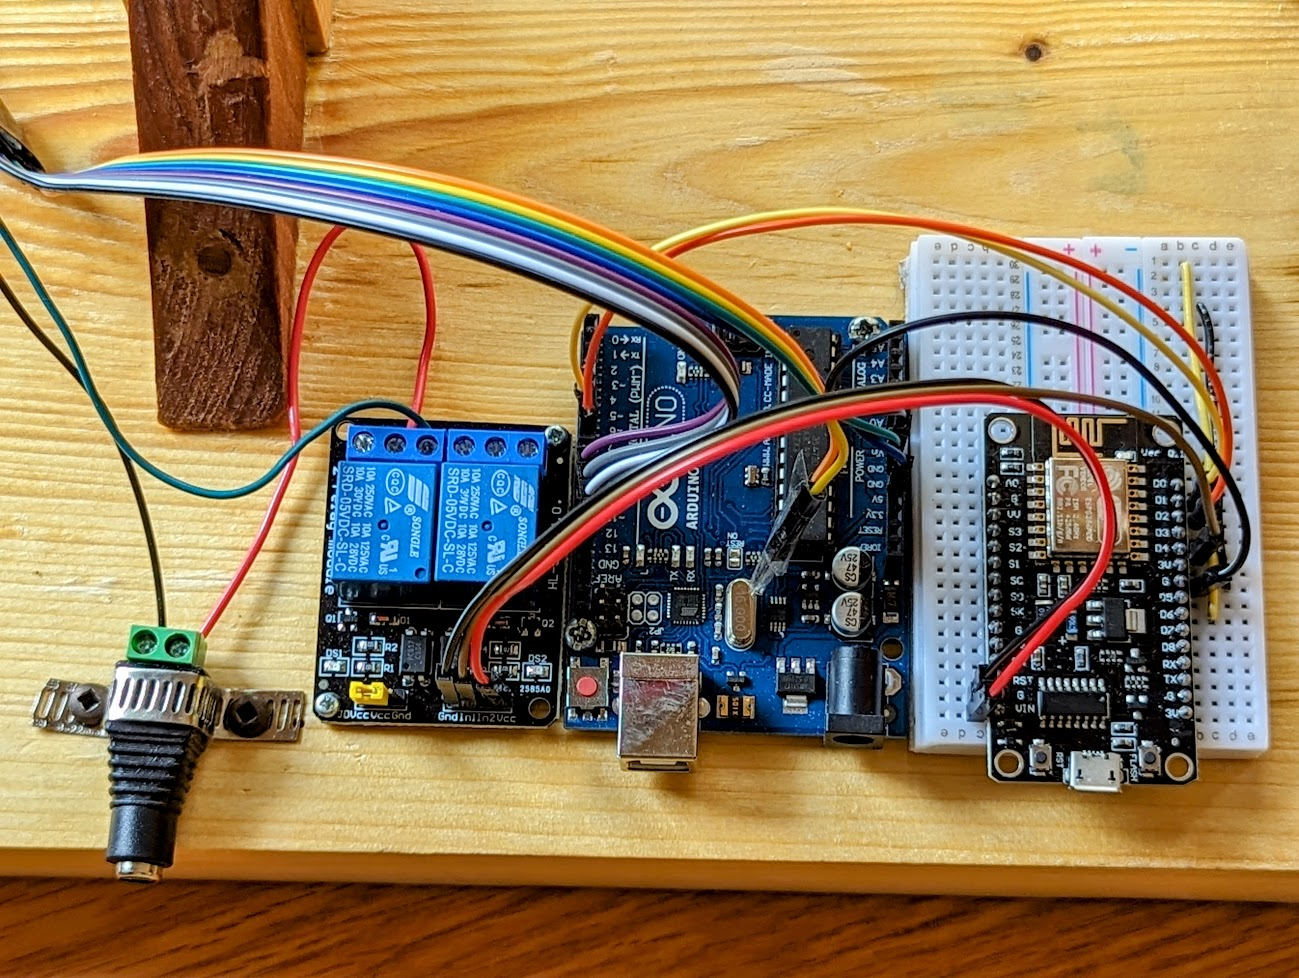
\includegraphics[width=0.8\linewidth]{Port-E_door05.jpg}
\caption{ Composants électroniques}
\end{figure}

\end{block}

%----------------------------------------------------------------------------------------
%	MÉTHODOLOGIE - METHODS
%----------------------------------------------------------------------------------------

\begin{block}{Méthodologie}

Pour réaliser cette expérimentation, nous avons mis en place un environnement de test comprenant un site web d'entreprise et un système de contrôle d'accès à des portes physiques. Les employés choisis ont été invités à utiliser leur portefeuille numérique pour s'authentifier sur le site web et pour déverrouiller les portes.

Les 4 étapes de cette expérimentation sont :
\begin{enumerate}
    \item Vous vous auto-attestez en tant que telle personne.
    \item Vous démontrez que vous avez le contrôle de votre boîte de courriel.
    \item Vous utilisez ces attestations vérifiables (Port-E) pour avoir accès à des services électroniques.
    \item Vous utilisez ces attestations vérifiables (Port-E) pour avoir accès à des emplacements physiques.
\end{enumerate}

\begin{figure}
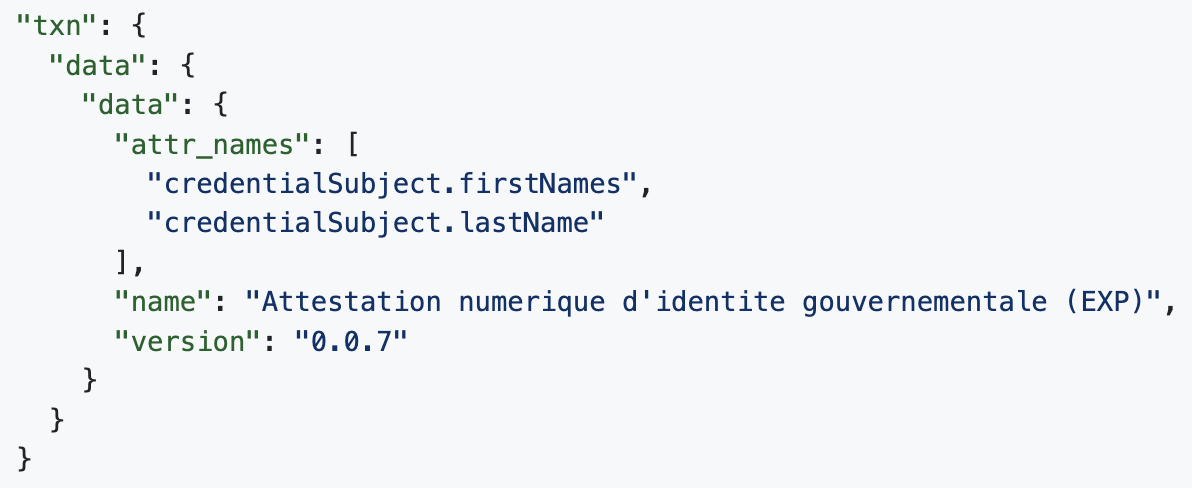
\includegraphics[width=1.0\linewidth]{Port-E_data01.png}
\caption{ L'attestation vérifiable auto-déclarée d'identité numérique} 
\end{figure}

\begin{figure}
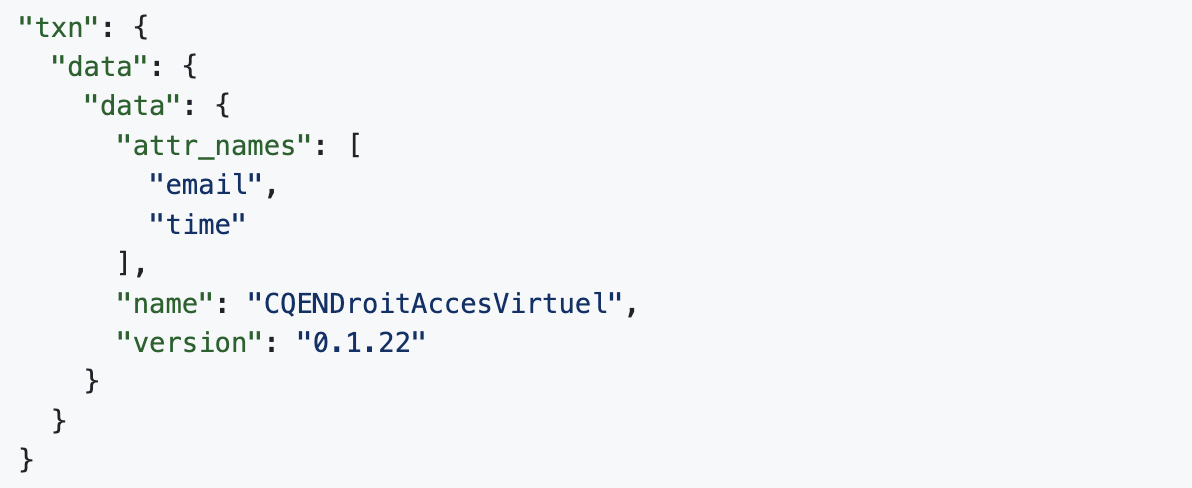
\includegraphics[width=1.0\linewidth]{Port-E_data02.png}
\caption{ L'attestation de preuve de contrôle de sa boîte de courriel} 
\end{figure}

\end{block}

\end{column} % End of the first column


\begin{column}{\sepwid}\end{column} % Empty spacer column

\begin{column}{\twocolwid} % Begin a column which is two columns wide (column 2)

%----------------------------------------------------------------------------------------
%	CAS D'UTILISATION - USE CASE
%----------------------------------------------------------------------------------------

\begin{alertblock}{Cas d'utilisation}
Le cas d'utilisation d'une attestation vérifiable pour un employé est un exemple intéressant et concret qui apporte une belle complexité. Les cas d'utilisation minimaux ont été élaborés afin de permettre la mise en place de toutes les composantes nécessaires pour expérimenter le concept sans toutefois résoudre les contraintes et particularités d'un cas d'affaires concret.

Sarah, notre employée, utilise son portefeuille numérique et obtient les attestations nécessaires qui prouvent son identité et son lien d'emploi. Par la suite, elle peut accéder au site web utilisé dans le cadre de son travail et également déverrouiller les portes d’accès sur les lieux de travail. 

\textit{Nous disons au revoir aux mots de passe oubliés et à la nécessité de répondre à plusieurs questions pour s’authentifier auprès d’un prestataire de services.}

\begin{figure}
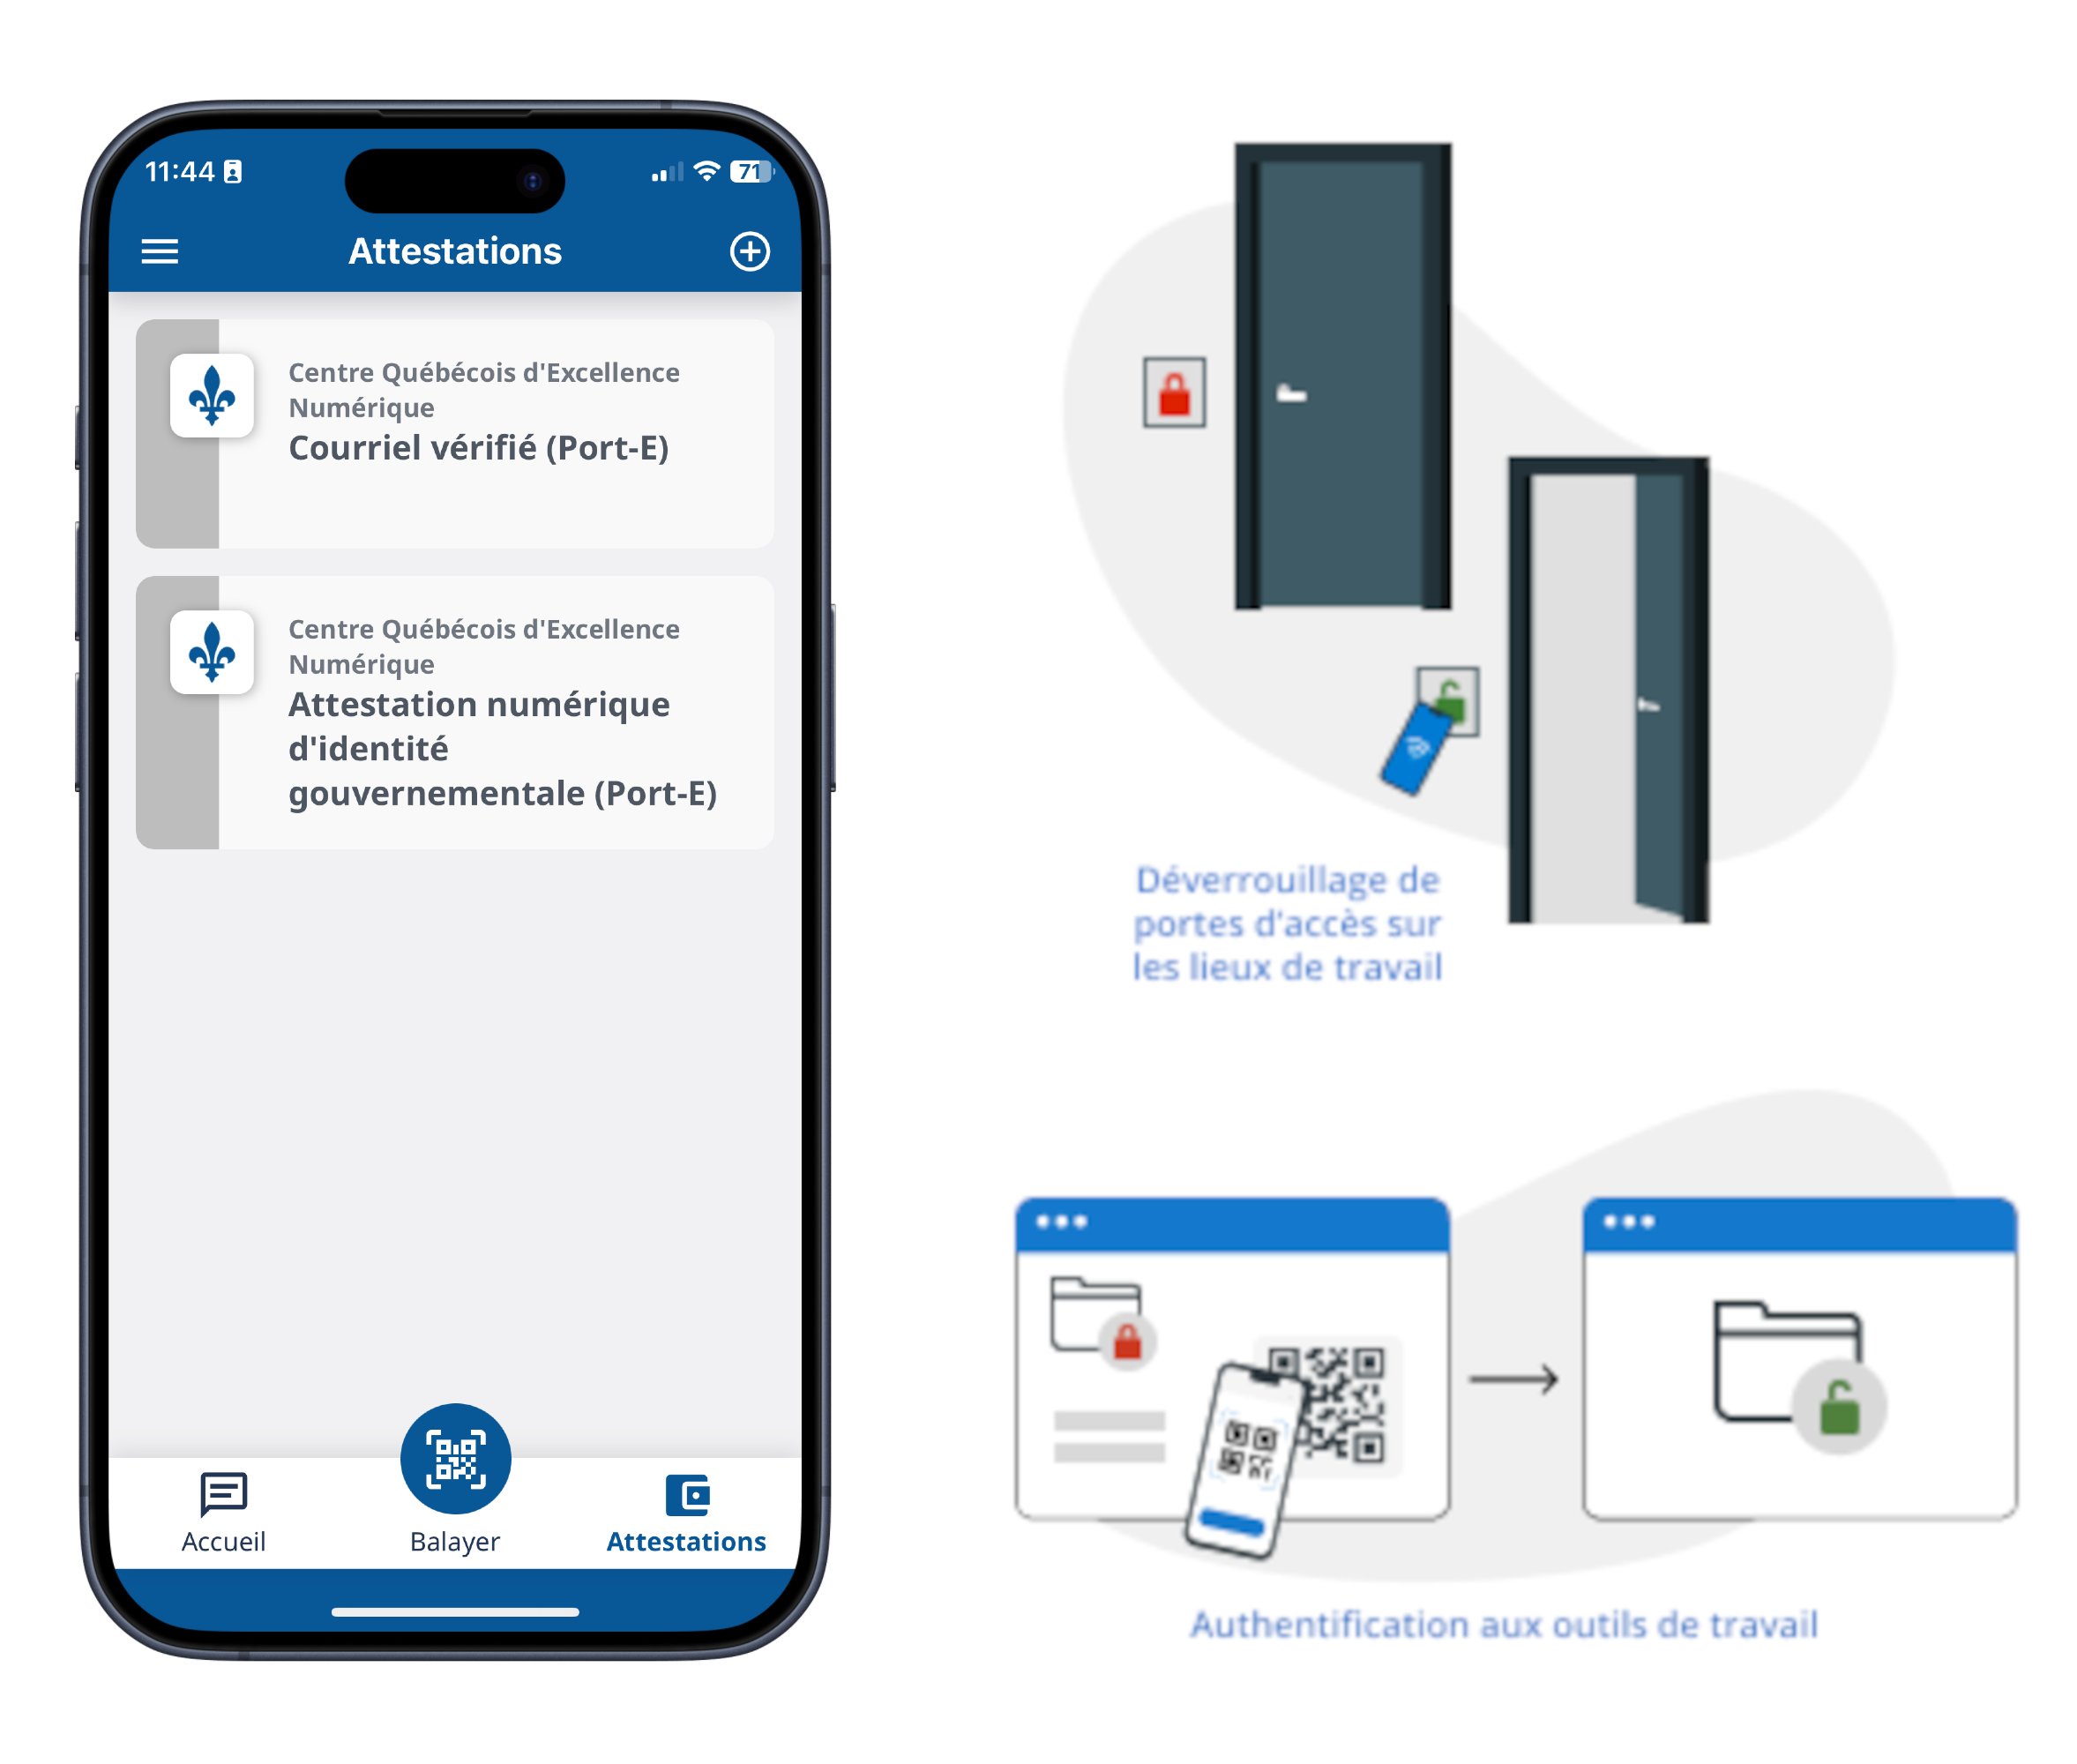
\includegraphics[width=0.5\linewidth]{Port-E-Usecase.png}
\caption{ Cas d'utilisation Port-E}
\end{figure}

\end{alertblock} 

\begin{figure}
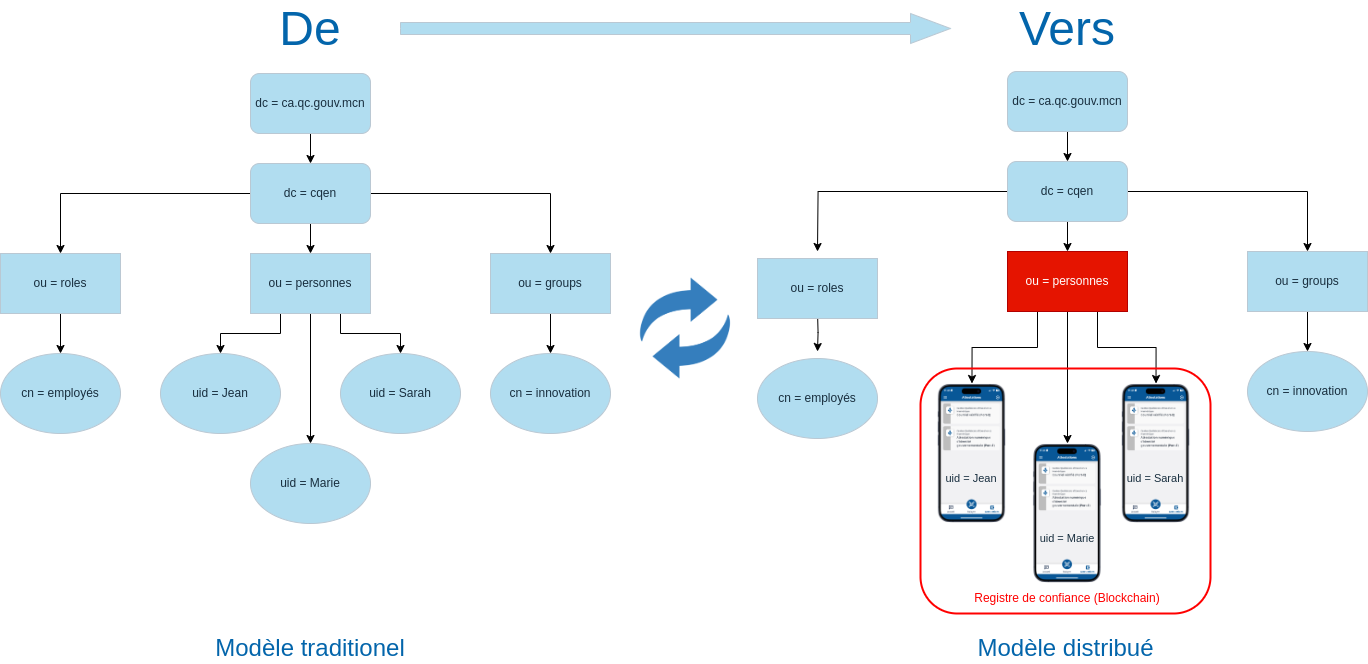
\includegraphics[width=0.9\linewidth]{Port-E-LDAP.png}
\caption{ Modèle de données d'accès}
\end{figure}

%----------------------------------------------------------------------------------------

\begin{columns}[t,totalwidth=\twocolwid] % Split up the two columns wide column again

\begin{column}{\onecolwid} % The first column within column 2 (column 2.1)


%----------------------------------------------------------------------------------------
%	RÉSULTATS - RESULTS
%----------------------------------------------------------------------------------------

\begin{block}{Résultats}

À la fin de cette expérimentation, nous avons obtenu des retours d'expérience de la part des employés sur l'utilisation du portefeuille numérique. Ces retours ont aidé à comprendre les avantages et les inconvénients de cette approche, et à identifier les améliorations potentielles.

Concrètement, deux schémas d'attestation vérifiables sont disponibles dans le portefeuille mobile de l'employé. Ils ont pour objectif de permettre :

\begin{enumerate}
\item L'émission de l'attestation d'identité.
    \begin{itemize}
        \item d'identifier le sujet de l'attestation.
    \end{itemize}

\item L'émission de l'attestation de courriel.
    \begin{itemize}
        \item d'identifier la boîte de courriel sur laquelle l'employé démontre un contrôle ;
        \item d'établir le lien entre la personne détentrice du courriel et son lien d'emploi lorsque la boîte de courriel est professionnelle.
    \end{itemize}

\item La vérification permet de valider.
    \begin{itemize}
        \item l'émission d'une requête de présentation exigeant la présentation des valeurs des attributs de l'attestation d'identité de Sarah ;
        \item la présentation du courriel professionnel dont Sarah a le contrôle.
    \end{itemize}
\end{enumerate}

\end{block}


%----------------------------------------------------------------------------------------
%	MENACE POUR LA VALIDITÉ - THREAT TO VALIDITY 
%----------------------------------------------------------------------------------------


\begin{block}{Menace pour la validité}
% \item \textbf{Menage à la valitité externe:} sont des facteurs qui affectent la généralisabilité des résultats. L'expérimentation


\begin{itemize}
    \item \textbf{Menace pour la validité interne:} sont des facteurs qui peuvent affecter des variables indépendantes ou qui n'ont pas été prises en compte lors de l'expérimentation. Certaines fonctionnalités qui ne sont pas le sujet final de l'expérimentation, telles comme les intéractions avec un système de gestion d'identité et d'accès ou les intéractions avec des panneaux de contrôle de porte réelles ont été simulées avec le but de réduire la complexité de l'implémentation.  
    
\end{itemize}
    
\end{block}

%----------------------------------------------------------------------------------------

\end{column} % End of column 2.1


\begin{column}{\onecolwid} % The second column within column 2 (column 2.2)

%----------------------------------------------------------------------------------------
%	PERSPECTIVES ET TRAVAUX FUTURS - PROSPECTS AND FURTHER WORK 
%----------------------------------------------------------------------------------------

%\setbeamercolor{block alerted title}{fg=black,bg=norange} % Change the alert block title colors
%\setbeamercolor{block alerted body}{fg=black,bg=white} % Change the alert block body colors

\begin{alertblock}{Perspectives et travaux futures}

\begin{itemize}

\item \textbf{L'intelligence artificielle} (IA) et la \textbf{blockchain} jouent un rôle crucial dans la \textbf{transformation numérique} de \textbf{l'administration publique}. Nous devons expérimenter ces technologies dans nos processus internes pour mieux comprendre leur potentiel et leurs défis avant de les appliquer à grande échelle dans les services publics. 

\item La \textbf{sécurité} et la \textbf{confidentialité des données} sont des préoccupations majeures dans l'application de {l'IA} et de la \textbf{blockchain}. Nous devons protéger les données personnelles et assurer la sécurité des systèmes contre les menaces potentielles. Les blockchains d'identité visent surtout à préserver la confidentialité des données personnelles, n'enregistrant que des \textbf{empreintes} des données réelles "\textit{on-chain}", tout en conservant les vraies données "\textit{off-chain}", dans les dispositifs des utilisateurs. 

\item L'IA peut être utilisée pour améliorer la \textbf{gestion des bâtiments intelligents}, optimiser l'utilisation de l'énergie et améliorer le confort des occupants; l'utilisation de caméras pour s'assurer qu'un employé n'a pas été suivi par une autre personne lors de son accès. Cela pourrait améliorer la sécurité tout en minimisant les inconvénients pour les employés.

\item L'évaluation de la \textbf{mise à l'échelle} de l'expérimentation sera réalisée ultérieurement, en tenant compte de la complexité des \textbf{environnements technologiques} et des {processus d'affaires} qui seront alors évalués en collaboration avec les équipes de réalisation.

\end{itemize}

\end{alertblock}

%----------------------------------------------------------------------------------------

\end{column} % End of column 2.2

\end{columns} % End of the split of column 2

\begin{column}{\twocolwid} % Begin a column which is two columns wide (column 2)

%----------------------------------------------------------------------------------------
%	IMAGES
%----------------------------------------------------------------------------------------

\begin{figure}
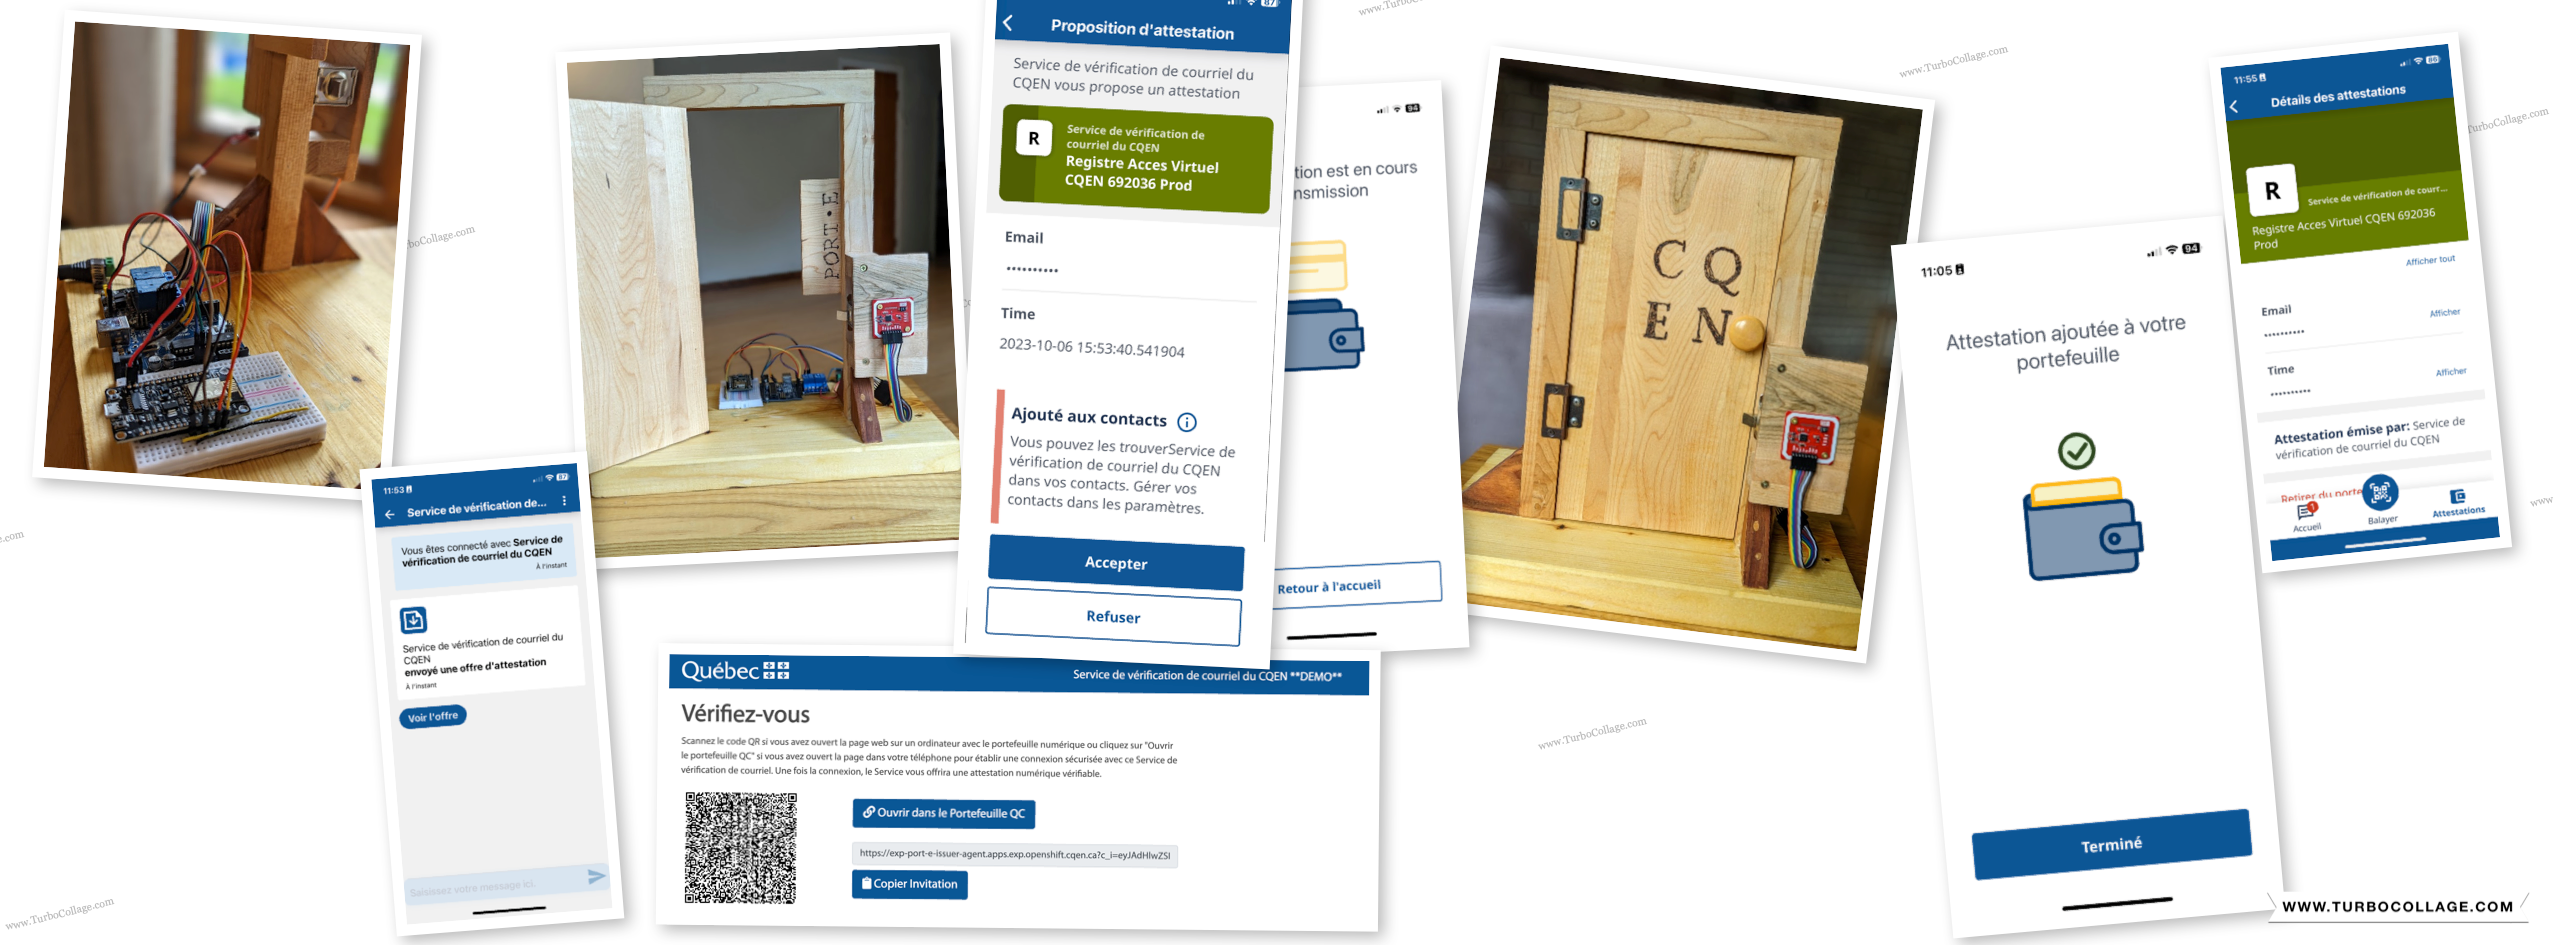
\includegraphics[width=0.8\linewidth]{Collage_02.png}
\caption{Certains visuels sur l'expérimentation}
\end{figure}

%----------------------------------------------------------------------------------------

\end{column} % End of last two column

\end{column} % End of the second column


\begin{column}{\sepwid}\end{column} % Empty spacer column

\begin{column}{\onecolwid} % The third column

%----------------------------------------------------------------------------------------
%	IMAGE ATTESTATION NUMÉRIQUE
%----------------------------------------------------------------------------------------

%\begin{figure}
%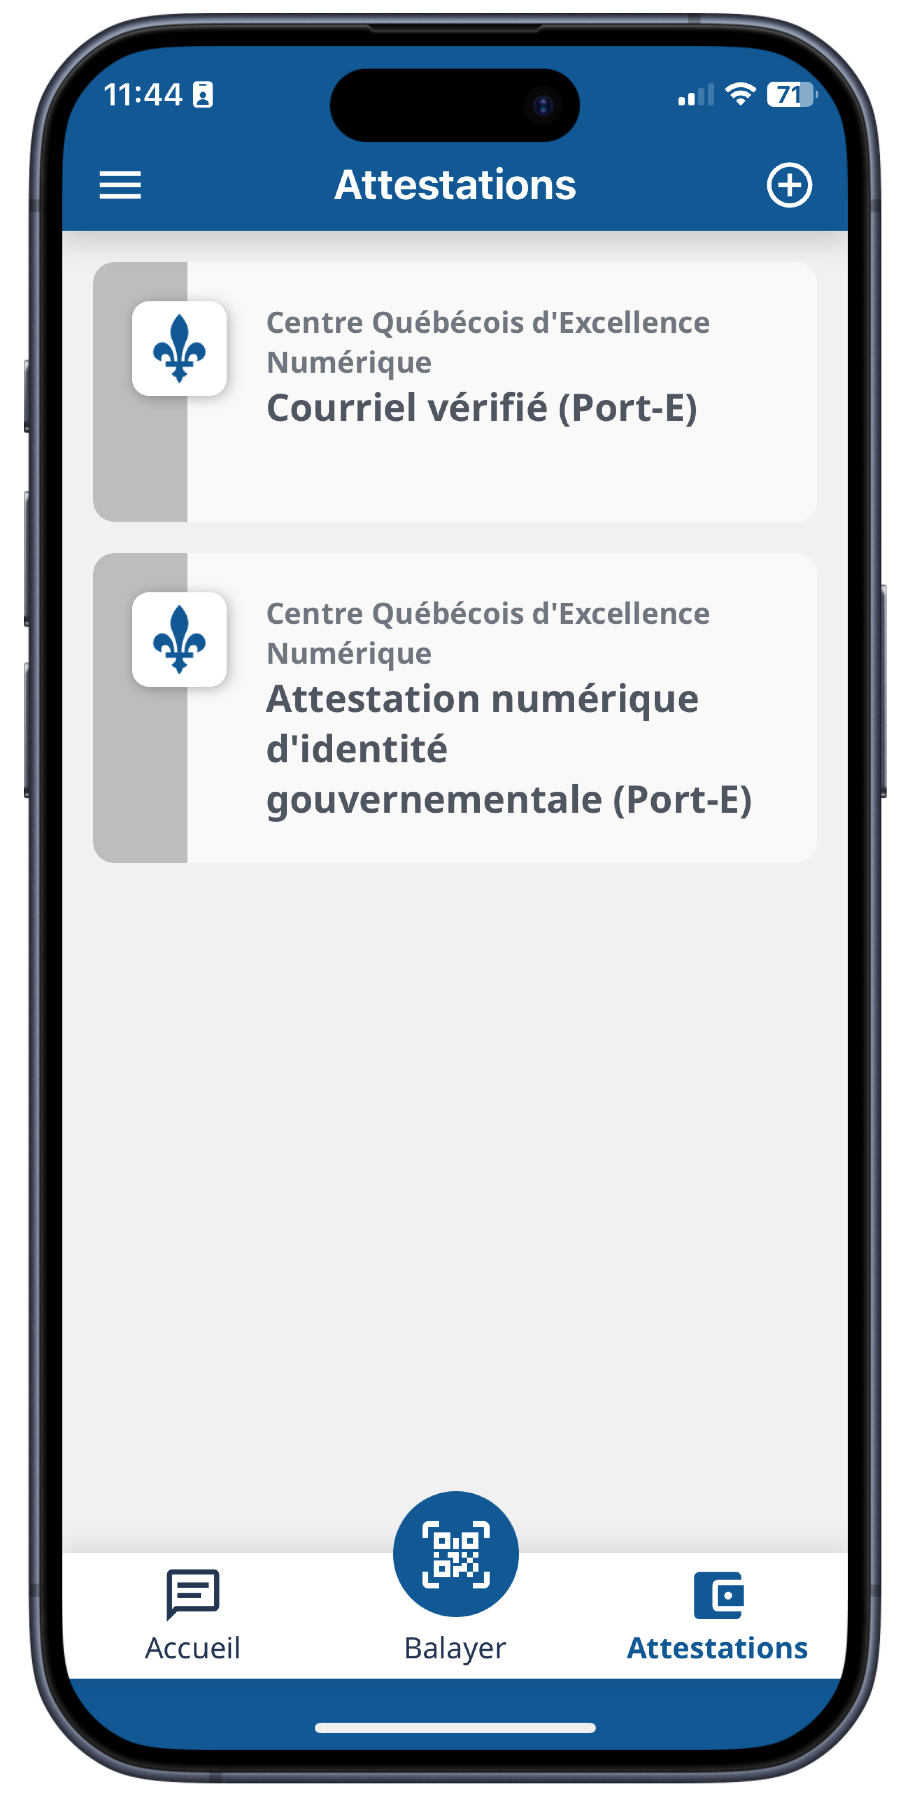
\includegraphics[width=0.6\linewidth]{attestation_portefeuille.png}
%\caption{Application mobile de portefeuille numérique}
%\end{figure}

%----------------------------------------------------------------------------------------
%	CONCLUSION
%----------------------------------------------------------------------------------------

\begin{block}{Conclusion}

L'expérimentation a démontré que l'usage d'un portefeuille numérique par les employés dans un environnement contrôlé d'expérimentation est non seulement réalisable, mais aussi très pratique. 

L'expérimentation a permis d'explorer les aspects techniques du contrôle d'accès aux ressources, tant virtuelles que physiques, et d'évaluer les modèles soutenant ce contrôle. Le courriel a été utilisé comme preuve du lien d'emploi, car l'employeur connaît cette relation et a déjà identifié au préalable l'employé. 

L'organisation émet une attestation vérifiable prouvant ce lien. L'accès physique a présenté des défis, notamment la taille des paquets NFC, résolus en utilisant un URL shortener. 

En conclusion, l'utilisation d'un portefeuille numérique pour les employés est relativement simple dans un environnement d'expérimentation, car les règles d'utilisation sont déjà bien définies. L'identité numérique facilite l'application de ces règles.

Par contre, les conclusions tirées de cette expérimentation doivent être prises en compte avec prudence lors de la mise en œuvre d'une application réelle. 

\end{block}

%----------------------------------------------------------------------------------------
%	INFORMATION ADDITIONELLE - ADDITIONAL INFORMATION
%----------------------------------------------------------------------------------------

\begin{block}{Information Additionelle}
Le prototype utilise la blockchain pancanadienne que nous opérons le Québec, l’Ontario et la Colombie-Britannique basé sur la technologie Hyperledger Indy.

Nous avons utilisé un portefeuille numérique pré-configuré dans le prototype basé sur les technologies Hyperledger Aries Framework Javascript (AFJ) et Hyperledger Aries Mobile Agent React Native (Bifold).

\end{block}

%----------------------------------------------------------------------------------------
%	RÉFÉRENCES - REFERENCES
%----------------------------------------------------------------------------------------

\begin{block}{Références}

\nocite{*} % Insert publications even if they are not cited in the poster
\small{\bibliographystyle{unsrt}
\bibliography{RefBiblio}\vspace{0.75in}}

\end{block}

%----------------------------------------------------------------------------------------
%	REMERCIEMENTS - ACKNOWLEDGEMENTS
%----------------------------------------------------------------------------------------

\setbeamercolor{block title}{fg=red,bg=white} % Change the block title color

\begin{block}{Remerciements}

\small{\rmfamily{Un grand merci à toutes les personnes et projets de code source libre dont le code a été utilisé.
Merci à la Colombie-Britannique pour l'inspiration.}} \\

\begin{figure}
\includegraphics[width=0.8\linewidth]{Port-E-Equipe.png}
\caption{L'équipe : Notre collègue Ricardo Cantu était absent lors de la photo, un grand merci à Ricardo pour avoir été l'ébéniste qui a construit la porte physique !}
\end{figure}

% \small{\rmfamily{Nam mollis tristique neque eu luctus. Suspendisse rutrum congue nisi sed convallis. Aenean id neque dolor. Pellentesque habitant morbi tristique senectus et netus et malesuada fames ac turpis egestas.}} \\

\end{block}

%----------------------------------------------------------------------------------------
%	COORDONNÉES - CONTACT INFORMATION
%----------------------------------------------------------------------------------------

\setbeamercolor{block alerted title}{fg=black,bg=norange} % Change the alert block title colors
\setbeamercolor{block alerted body}{fg=black,bg=white} % Change the alert block body colors

\begin{alertblock}{Coordonnées}

\begin{itemize}
% \item Web: \href{https://www.quebec.ca/gouvernement/ministere/cybersecurite-numerique}{https://www.quebec.ca/gouvernement/ministere/cybersecurite-numerique}
% \item GitHub: \href{https://github.com/CQEN-QDCE}{https://github.com/CQEN-QDCE}
\item Email: \href{mailto:cqen@mcn.gouv.qc.ca}{cqen@mcn.gouv.qc.ca}
\end{itemize}

\end{alertblock}

% Ajouter de l'espace afin de repousser le logo du MCN complètement en bas du poster
\vspace{15cm}

\begin{center}
\begin{tabular}{ccc}

\includegraphics[width=1.0\linewidth]{mcn.png}
\end{tabular}
\end{center}

%----------------------------------------------------------------------------------------

\end{column} % End of the third column

\end{columns} % End of all the columns in the poster

\end{frame} % End of the enclosing frame

\end{document}
